This study employs an autoethnographic research-creation design with collaborative through-ways and bypasses, organized by the Speculocultural Technopoietic cycle—\emph{Unsettling} (U), \emph{Remixing} (R), \emph{Embodying} (E), and \emph{Transmitting} (T). More conventional methods (autoethnography, critical technical practice, reflective/speculative design, participatory co-design) are integrated within specific protocols and procedures of ST.

\subsection{Conceptual and Theoretical Background}

\subsubsection{Core Premise}
\enquote{
	Speculocultural Technopoiesis is the process in which cultural speculation guides embodied technological modification and practice to generate new forms of knowledge.}

\vspace{1.0em}

\textbf{Speculocultural:} speculative reimagining through specific cultural epistemologies.

\textbf{Technopoiesis:} knowledge creation through embodied making and material manipulation.

\subsubsection{Conceptual Architecture}

	\begin{figure}[H]
		\centering
		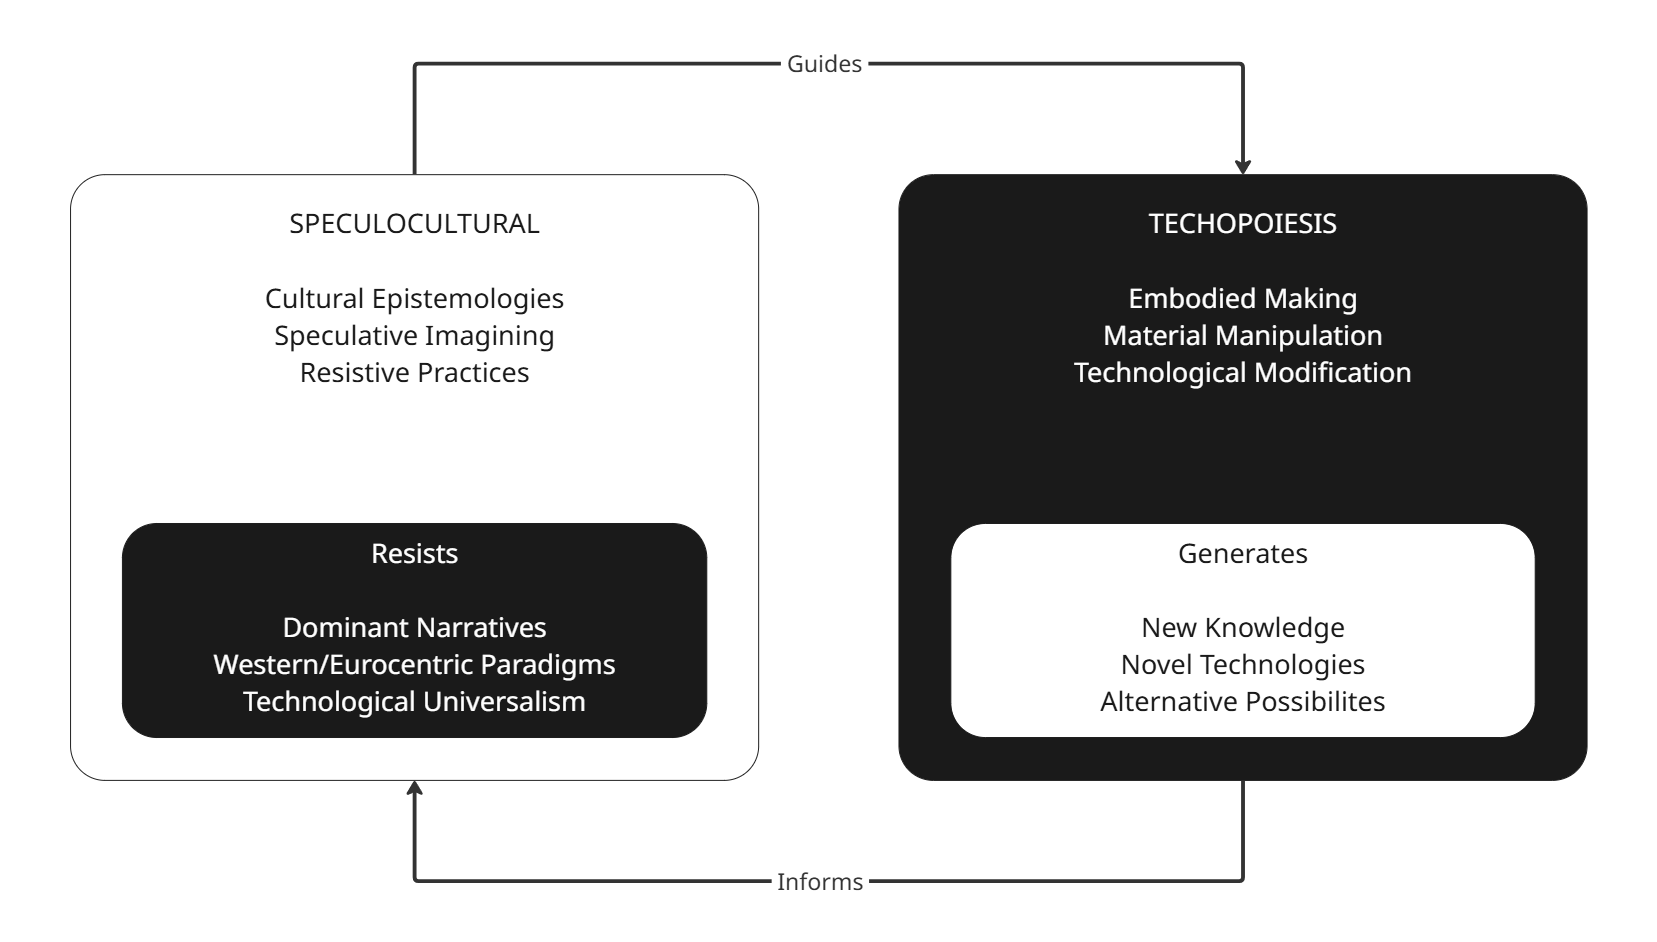
\includegraphics[width=.85\textwidth]{assets/figures/st_architecture.png}
		\caption{Two main components of Speculocultural Technopoiesis}
		\label{fig:concept-architecture}
	\end{figure}


\subsubsection{The Foundational Relationship}
\textbf{Speculocultural}

Marginalized communities often use speculative narratives as sites of resistance, imagining alternative technological futures through their specific cultural lenses. The function of such speculation is to strategically reveal the ways in which various forms of domination render marginalized perspectives invisible. All the while simultaneously pushing to the margins.

\textbf{Technopoiesis}

Knowledge emerges through cyclical processes of embodied material manipulation and technological modification. These novel understandings arise from hands-on emergent engagements, discovering what becomes possible when tools are approached through different epistemological backgrounds.

\textbf{Integration}

Speculocultural imagination guides technopoietic practice by providing cultural grounding and imaginative direction for technological practices and potential modifications of those technologies. This ensures that embodied work serves to both resist and codify in an effort to stop reproducing dominant paradigms and providing only  "technical fixes." Technopoietic knowledge informs speculocultural narratives by generating new forms of technological knowledge through embodied practice and nascent procedural habit. This grounds cultural imagination in material technological possibilities discovered through these practices.

